\documentclass[aspectratio=169,usenames,dvipsnames]{beamer}

% fonts
%\usepackage[T1]{fontenc}
%\usepackage[utf8]{inputenc}

%\usefonttheme{professionalfonts} % using non standard fonts for beamer
\usefonttheme{serif} % default family is serif

\usepackage{palatino}
%\usepackage{gfsartemisia}
%\usepackage{theanooldstyle}

\usepackage{euscript}	 % Шрифт Евклид
\usepackage{mathrsfs} % Красивый матшрифт
\usepackage{amssymb}
\usepackage{bm}
\usepackage{calc} % perform arithmetic on the arguments
\usepackage{cancel} % cancelling things
\usepackage{marvosym} % fancy arrow
\usepackage[ruled,vlined]{algorithm2e}
\usepackage{algorithmic}

\definecolor{mygreen}{HTML}{348A41}  % 53945D
\definecolor{myred}{HTML}{B73239} 
\definecolor{myorange}{HTML}{AB5F1F}  % 805129
\definecolor{mypurple}{HTML}{533E8F} 
\definecolor{myblack}{HTML}{4C4848} 
\definecolor{mygrey}{HTML}{F4EDE0} %  F5F1EA

\usepackage{epstopdf}
\usepackage{xcolor}

% adding images
\usepackage{graphicx} 
\usepackage{tcolorbox}

% for ul
\usepackage{soul}

% adding gifs
\usepackage{animate}

% positioning textblocks
\usepackage[absolute, overlay]{textpos} 
\textblockorigin{0mm}{0mm} % start everything near the top-left corner

% Работа с русским языком
\usepackage{cmap}					% поиск в PDF
%\usepackage{mathtext} 				% русские буквы в фомулах
%\usepackage[T2A]{fontenc}			% кодировка
%\usepackage[utf8]{inputenc}			% кодировка исходного текста

% Дополнительная работа с математикой
%\usepackage{amsmath,amsfonts,amssymb,amsthm,mathtools} % AMS
%\usepackage{icomma} % "Умная" запятая: $0,2$ --- число, $0, 2$ --- перечисление

%% Номера формул
%\mathtoolsset{showonlyrefs=true} % Показывать номера только у тех формул, на которые есть \eqref{} в тексте.

% Работа с картинками
\usepackage{graphicx}  % Для вставки рисунков
\graphicspath{{figures/}}  % папки с картинками
\usepackage{wrapfig} % Обтекание рисунков и таблиц текстом

% drawing with tikz
\usepackage{tikz}
\usepackage{hf-tikz}
\usetikzlibrary{arrows}
\usetikzlibrary{shapes}
\usetikzlibrary{plotmarks}

\tikzset{
	treenode/.style = {align=center, inner sep=1.ex, minimum size=1cm,
		font=\sffamily},
	arn_n/.style = {treenode, rectangle, black, draw=black, minimum width = 0.05\textwidth, minimum height = 1 cm},% 
	level distance = 2.5cm,
	level 1/.style={sibling distance=16.cm},
	level 2/.style={sibling distance=8.cm},
	level 3/.style={sibling distance=3.7cm}
}

  \tikzset{
	invisible/.style={opacity=0},
	visible on/.style={alt=#1{}{invisible}},
	alt/.code args={<#1>#2#3}{%
		\alt<#1>{\pgfkeysalso{#2}}{\pgfkeysalso{#3}} % \pgfkeysalso doesn't change the path
	},
}

%% Работа с таблицами
%\usepackage{array,tabularx,tabulary,booktabs} % Дополнительная работа с таблицами
%\usepackage{longtable}  % Длинные таблицы
%\usepackage{multirow} % Слияние строк в таблице
%\renewcommand{\arraystretch}{1.3} %The height of each row is set to 1.5 relative to its default height. 

% Two ways of getting rid of total slides number

%\setbeamertemplate{footline}
%    {\begin{beamercolorbox}[sep=1ex]{author in head/foot}
%      \rlap{\textit{\insertshorttitle}}\hfill\insertauthor\hfill\llap{\insertframenumber}%
%      \end{beamercolorbox}%
%}

\makeatletter
\setbeamertemplate{footline}
{
	\leavevmode%
	\hbox{%
		\begin{beamercolorbox}[wd=.333333\paperwidth,ht=2.25ex,dp=1ex,center]{author in head/foot}%
			\usebeamerfont{author in head/foot}\insertshortauthor~~\beamer@ifempty{\insertshortinstitute}{}{\insertshortinstitute}
%            {(\insertshortinstitute)}
		\end{beamercolorbox}%
		\begin{beamercolorbox}[wd=.333333\paperwidth,ht=2.25ex,dp=1ex,center]{title in head/foot}%
			\usebeamerfont{title in head/foot}\insertshorttitle
		\end{beamercolorbox}%
		\begin{beamercolorbox}[wd=.333333\paperwidth,ht=2.25ex,dp=1ex,right]{date in head/foot}%
			\usebeamerfont{date in head/foot}\insertshortdate\hspace*{2em}
			\insertframenumber/\inserttotalframenumber\hspace*{2ex} 
	\end{beamercolorbox}}%
	\vskip0pt%
}
\makeatother

% Beamer presentation style
\mode<presentation> {
	\usetheme{Pittsburgh}
	\usecolortheme{dove}
	%\setbeamertemplate{footline} % To remove the footer line in all slides uncomment this line
	%\setbeamertemplate{footline}[page number] % To replace the footer line in all slides with a simple slide count uncomment this line
	%\setbeamertemplate{navigation symbols}{} % To remove the navigation symbols from the bottom of all slides uncomment this line
	
	%	\setbeamercolor{frametitle}{fg=white,bg=greyone}
	%	\setbeamercolor{titlelike}{parent=palette quaternary}
	
	%	\setbeamertemplate{frametitle}
	%	{
	%		\begin{textblock*}{\hsize}(.75\hsize,0.05\vsize)
	%			\begin{tcolorbox}[colframe=white, colback=mygrey, width=0.33\hsize,
	%				arc=2.mm, boxsep=2mm,
	%				box align=center,
	%				halign=center,
	%				valign=center,
	%				]
	%				\insertframetitle
	%			\end{tcolorbox}
	%		\end{textblock*}
	%	}
}

%% custom title
%\newcommand{\myframetitle}[3]{
%	\begin{textblock*}{\hsize}(#1,0.05\vsize)
%		\begin{tcolorbox}[colframe=white, colback=mygrey, width=#2,
%			arc=2.mm, boxsep=2mm,
%			box align=center,
%			halign=center,
%			valign=center,
%			]
%			\Large
%			#3
%		\end{tcolorbox}
%	\end{textblock*}
%}

% custom title
\newcommand{\myframetitle}[3]{
	\begin{textblock*}{#1}(#2,0.05\vsize)
		\begin{tcolorbox}[colframe=white, colback=mygrey, width=#1,
			arc=2.mm, boxsep=2mm,
			box align=center,
			halign=center,
			valign=center,
			]
			\Large
			\centering
			#3
		\end{tcolorbox}
	\end{textblock*}
}

% custom subtitle
\newcommand{\myframesubtitle}[2]{
	
	\begin{textblock*}{5cm}(#1,0.123\vsize)
		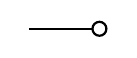
\begin{tikzpicture}
		\draw[thick,-o,black] (0.,0.) -- (1.0,0.);
		\end{tikzpicture}
	\end{textblock*}
	
	\begin{textblock*}{0.5\hsize}(#1+0.075\paperwidth,0.1\vsize)
		\normalsize
		\vspace{0.6mm}
		%		\centering
		#2
	\end{textblock*}
}

% new color for the bullet/subbullet
\newcommand{\mybullet}{$\textcolor{myblack}{\bullet}$}
\newcommand{\mysubbullet}{$\textcolor{myblack}{\circ}$}
\newcommand{\ev}{\mathbb{E}_{\text{p}(\bm x,y)}}
\newcommand{\pluseq}{\mathrel{+}=}

\newcommand{\beginbackup}{
   \newcounter{framenumbervorappendix}
   \setcounter{framenumbervorappendix}{\value{framenumber}}
}
\newcommand{\backupend}{
   \addtocounter{framenumbervorappendix}{-\value{framenumber}}
   \addtocounter{framenumber}{\value{framenumbervorappendix}} 
}

%----------------------------------------------------------------------------------------
%	TITLE PAGE
%----------------------------------------------------------------------------------------

\author[Sergey Korpachev]{Sergey Korpachev}%
%\author[Sergey Korpachev]{Sergey Korpachev\inst{1, 2} on behalf of Dépôt}%
\author[Sergey Korpachev]{Sergey Korpachev on behalf of Dépôt}
\institute[]{
%\institute[MIPT, LPI]{
%	\newline
%	\inst{1} {Moscow Institute of Physics and Technology}\\
%	\vspace{1mm}
%	\inst{2} {Lebedev Physical Institute of the Russian Academy of Sciences}\\
}
%\titlegraphic{
%	%\vspace{-.5cm}
%	%\hspace{1cm}
%	
\includegraphics[width=2.5cm]{mipt_logo.png}\hspace*{0.1cm}
%	
\includegraphics[width=1.5cm]{images/newLogoLPI.png}\hspace*{0.6cm}
%}

\title[Machine Learning (GitHub: SergeyKorpachev)]{}
%\date[\today]{}
\date[April 10, 2025]{}

%------------------------------------------------

\begin{document}

\begin{frame}
\centering
\huge

%\vspace{-0.3\paperheight}
\begin{tcolorbox}[colframe=white, colback=mygrey, width=0.45\paperwidth,
	arc=2.mm, boxsep=2mm,
	box align=center,
	halign=center,
	valign=center,
	]
	\Large
	Machine Learning: short introduction\\
    (trees and ANN),\\
    part 1
\end{tcolorbox}

\vspace{0.1\paperheight}
\centering
\large
\insertauthor\\

\scriptsize
\vspace{0.03\paperheight}
\hspace{0.17\paperwidth}
\insertinstitute

\vfill
\inserttitlegraphic
\transfade[duration=.4]
\end{frame}

%%------------------------------------------------
%------------------------------------------------
\section{Outline}
%------------------------------------------------
%------------------------------------------------

\begin{frame}[t]
\myframetitle{0.2\paperwidth}{0.04\paperwidth}{\insertsection}

\vspace{0.20\paperheight}
\begin{itemize}
    \centering
	\itemsep1.2ex
	\setbeamertemplate{items}{\mybullet}
	\item Machine learning (ML)
	\item Data
	\item Features in ML
	\item ML pipeline
	\item Linear model
	\item Decision tree
	\item Neural network
 	\item Summary
\end{itemize}

\transfade[duration=.4]
\end{frame}

%------------------------------------------------
%------------------------------------------------
\section{Machine learning}
%------------------------------------------------
%------------------------------------------------

\begin{frame}[plain]
\centering
\huge

%\begin{textblock*}{0.3\paperwidth}(0.25\paperwidth,0.3\paperheight)
\centering
\vspace{0.1\paperheight}
\begin{tcolorbox}[colframe=white, colback=mygrey, width=0.5\paperwidth,
	arc=2.mm, boxsep=2mm,
	box align=center,
	halign=center,
	valign=center,
	]
	\insertsection
\end{tcolorbox}

%\end{textblock*}

\transfade[duration=.4]
\end{frame}

%------------------------------------------------

\subsection{what is it?}
\begin{frame}

\myframetitle{0.35\paperwidth}{0.04\paperwidth}{\insertsection}
\myframesubtitle{0.37\paperwidth}{\insertsubsection}

\centering
\vspace{0.20\textheight}


\includegraphics[width=0.4\textwidth]{what_is_ml.png}
\only<2->{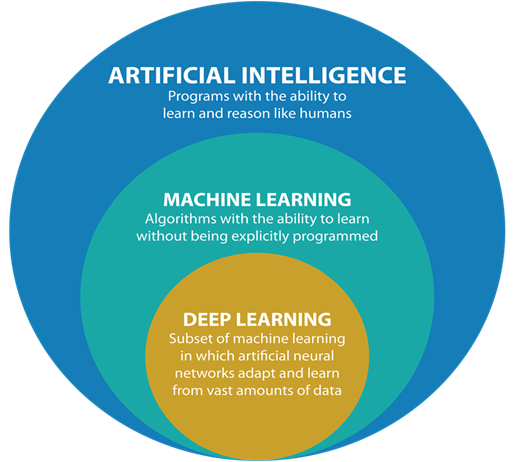
\includegraphics[width=0.27\textwidth]{ai_ml_dl.png}}
\hspace{0.07\textheight}
\only<3->{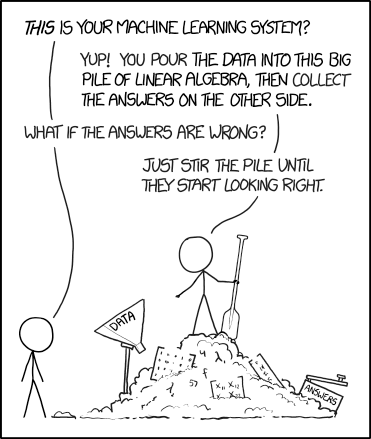
\includegraphics[width=0.25\textwidth]{approximation.png}}

\end{frame}

%------------------------------------------------

\subsection{The Fourth Paradigm (Tony Hey, ...)}
\begin{frame}
\myframetitle{0.35\paperwidth}{0.04\paperwidth}{\insertsection}
\myframesubtitle{0.37\paperwidth}{\insertsubsection}

\centering
\vspace{0.20\textheight}
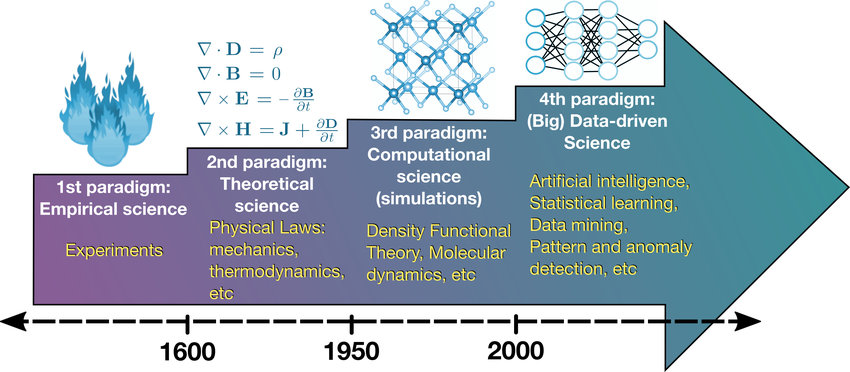
\includegraphics[width=1.0\textwidth]{science_paradigms.png}

\end{frame}

%------------------------------------------------
%------------------------------------------------
\section{Data}
%------------------------------------------------
%------------------------------------------------

\begin{frame}[plain]
\centering
\huge

%\begin{textblock*}{0.3\paperwidth}(0.25\paperwidth,0.3\paperheight)
\centering
\vspace{0.1\paperheight}
\begin{tcolorbox}[colframe=white, colback=mygrey, width=0.3\paperwidth,
	arc=2.mm, boxsep=2mm,
	box align=center,
	halign=center,
	valign=center,
	]
	\insertsection
\end{tcolorbox}

%\end{textblock*}

\transfade[duration=.4]
\end{frame}

%------------------------------------------------

\subsection{what is data?}
\begin{frame}

\myframetitle{0.27\paperwidth}{0.04\paperwidth}{\insertsection}
\myframesubtitle{0.29\paperwidth}{\insertsubsection}

\vspace{0.1\paperheight}
\begin{columns}
	\column{0.3\textwidth}
	Anything can be data:
	\begin{enumerate}
		\item Numbers
		\item Text
		\item Images
		\item Sound
		\item Geomap
		\item Particle collisions
		\item Knowledge
		\item You name it
	\end{enumerate}

	\column{0.7\textwidth}
	\begin{minipage}[c][.99\textheight][t]{\linewidth}
		\centering
		\vspace{0.2\paperheight}
		\begin{figure}[t]
			\centering
			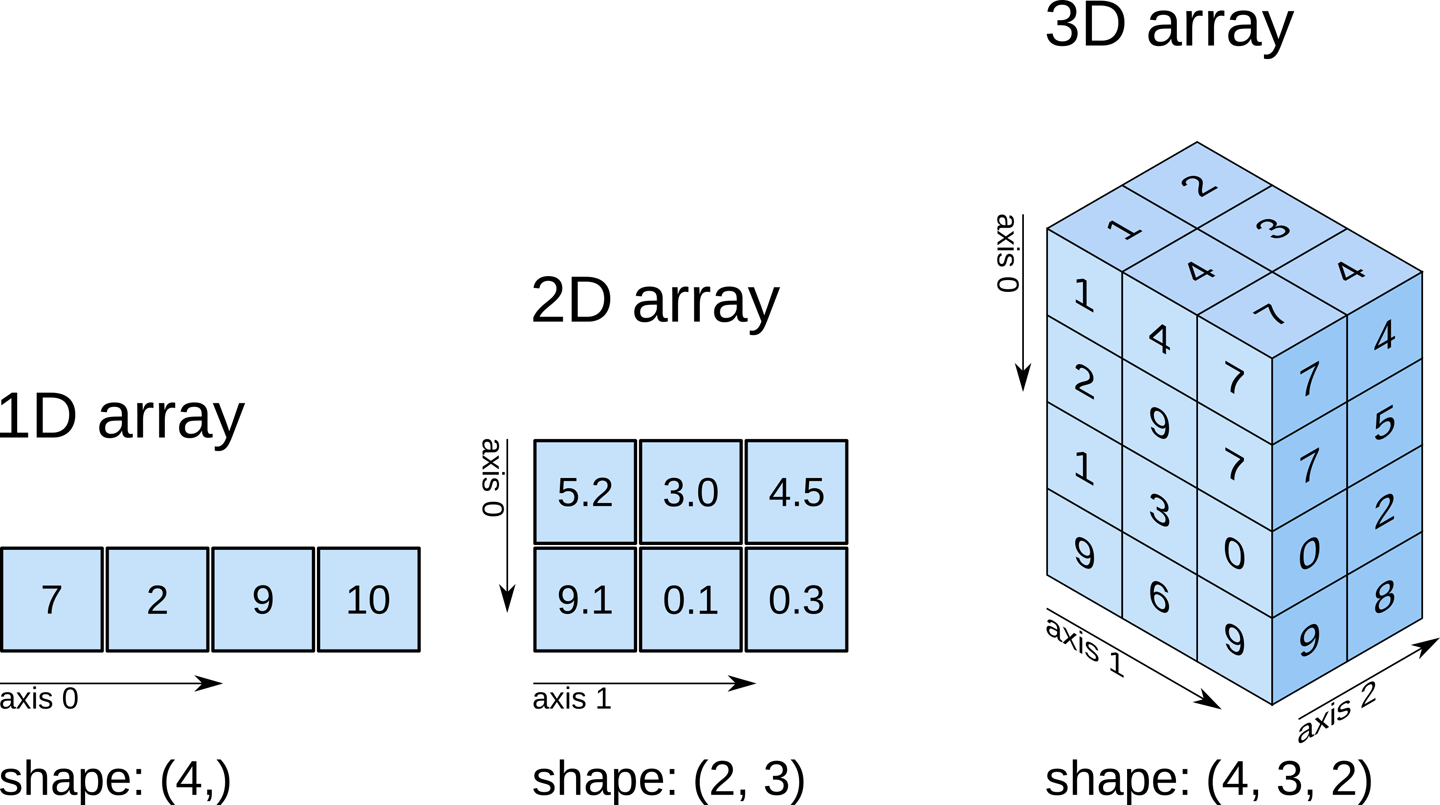
\includegraphics[width=0.4\linewidth]{numpy_array.png}
			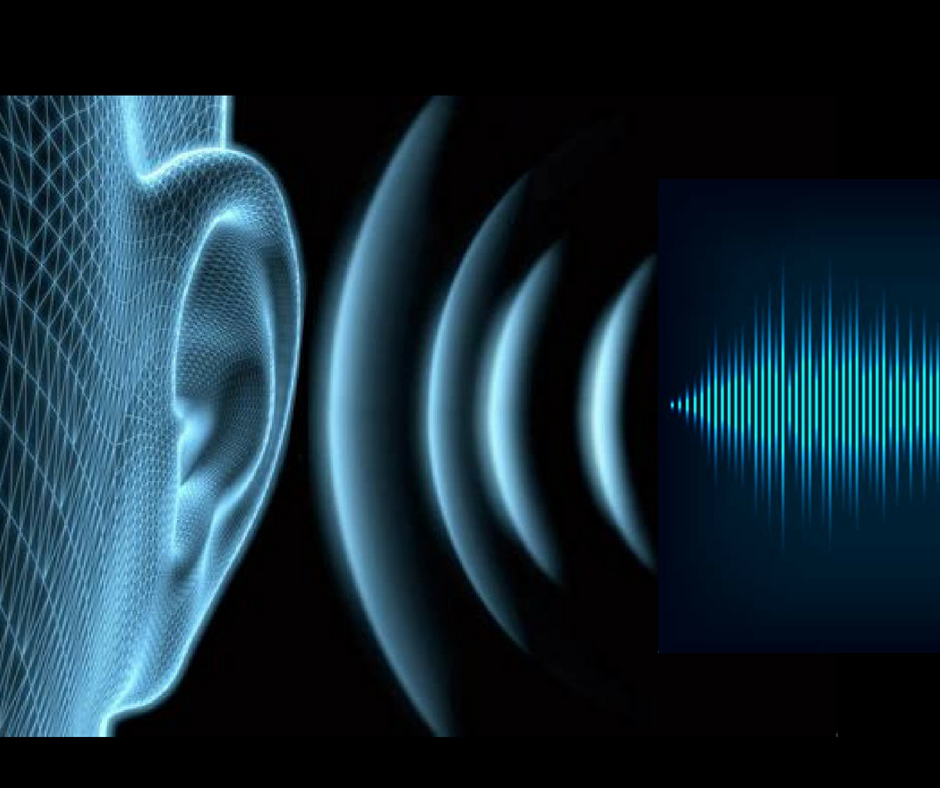
\includegraphics[width=0.25\linewidth]{sound}
			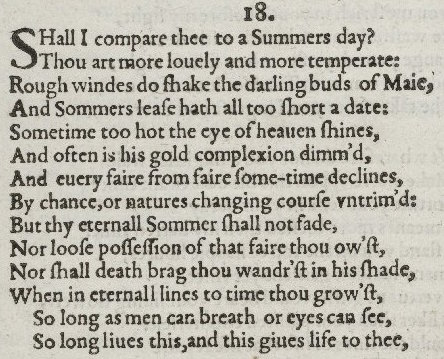
\includegraphics[width=0.2\linewidth]{Text}
			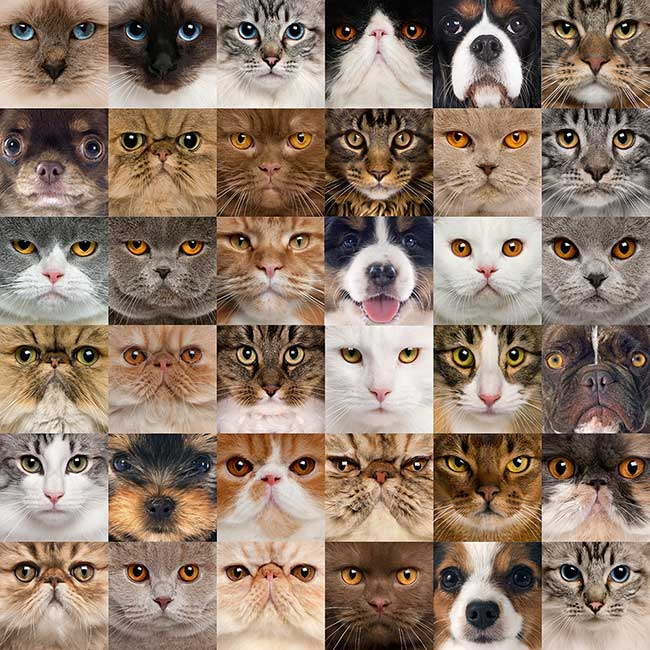
\includegraphics[width=0.25\linewidth]{cat}
			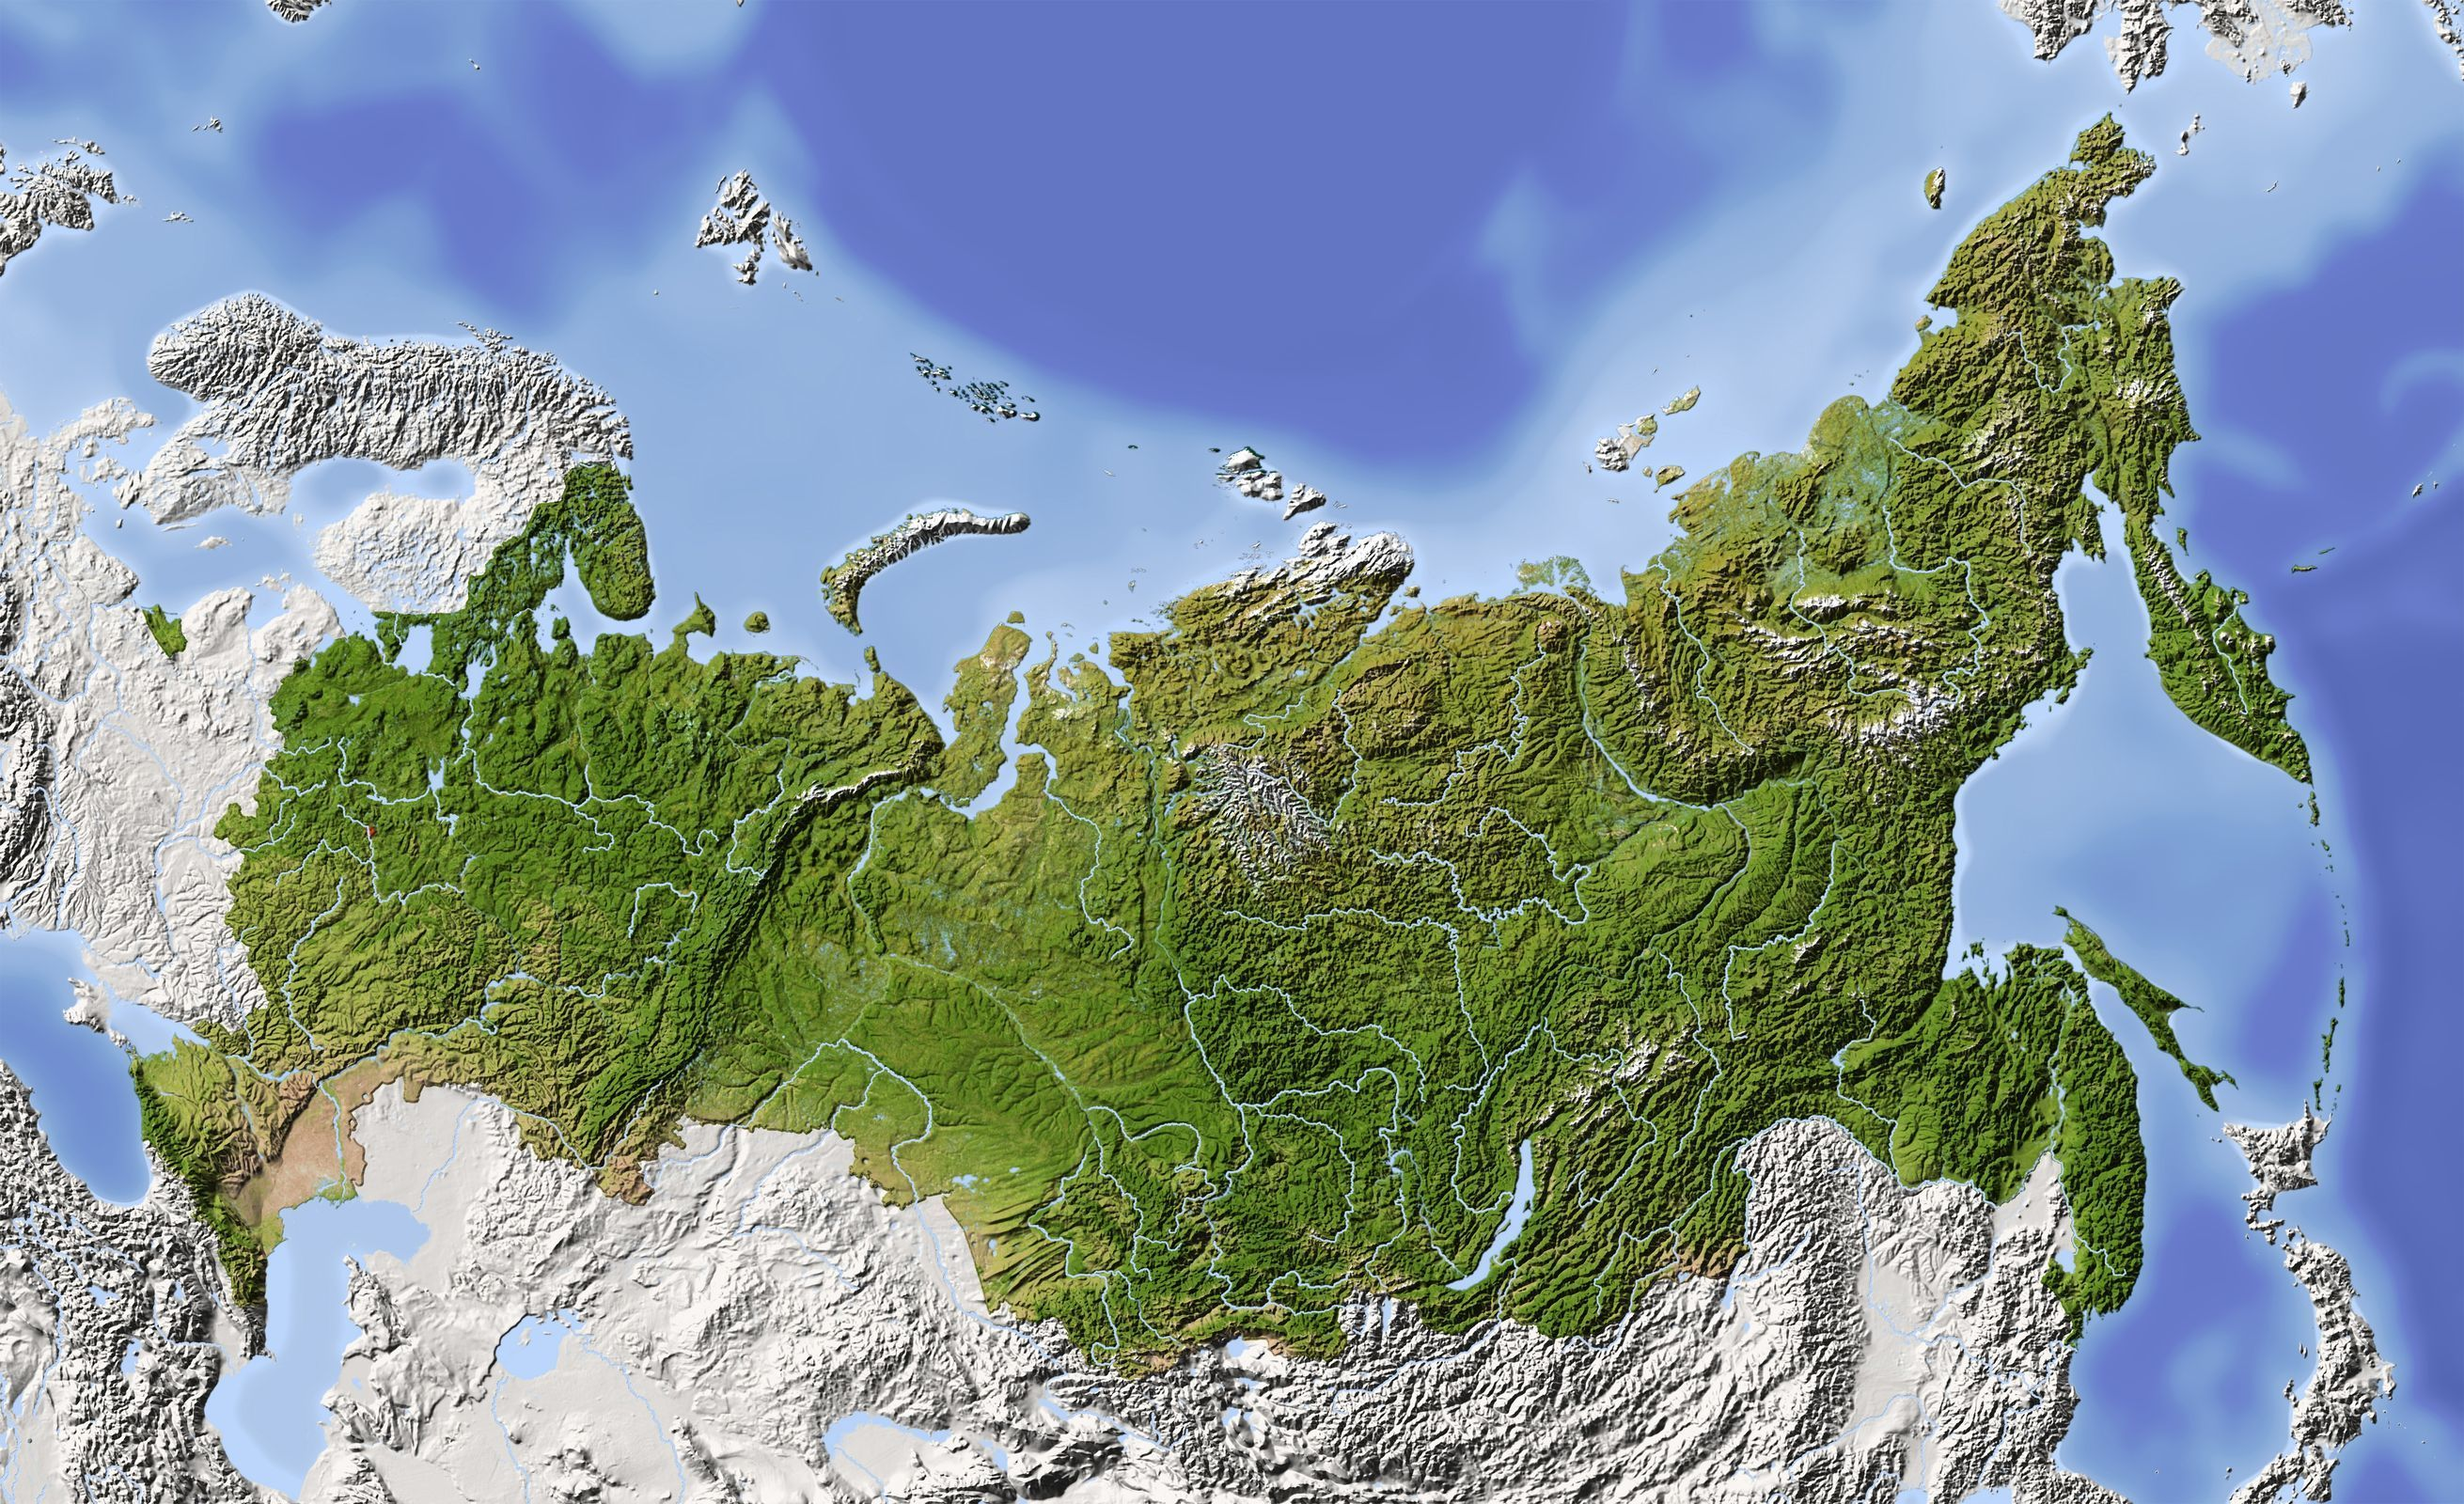
\includegraphics[width=0.3\linewidth]{geomap}
			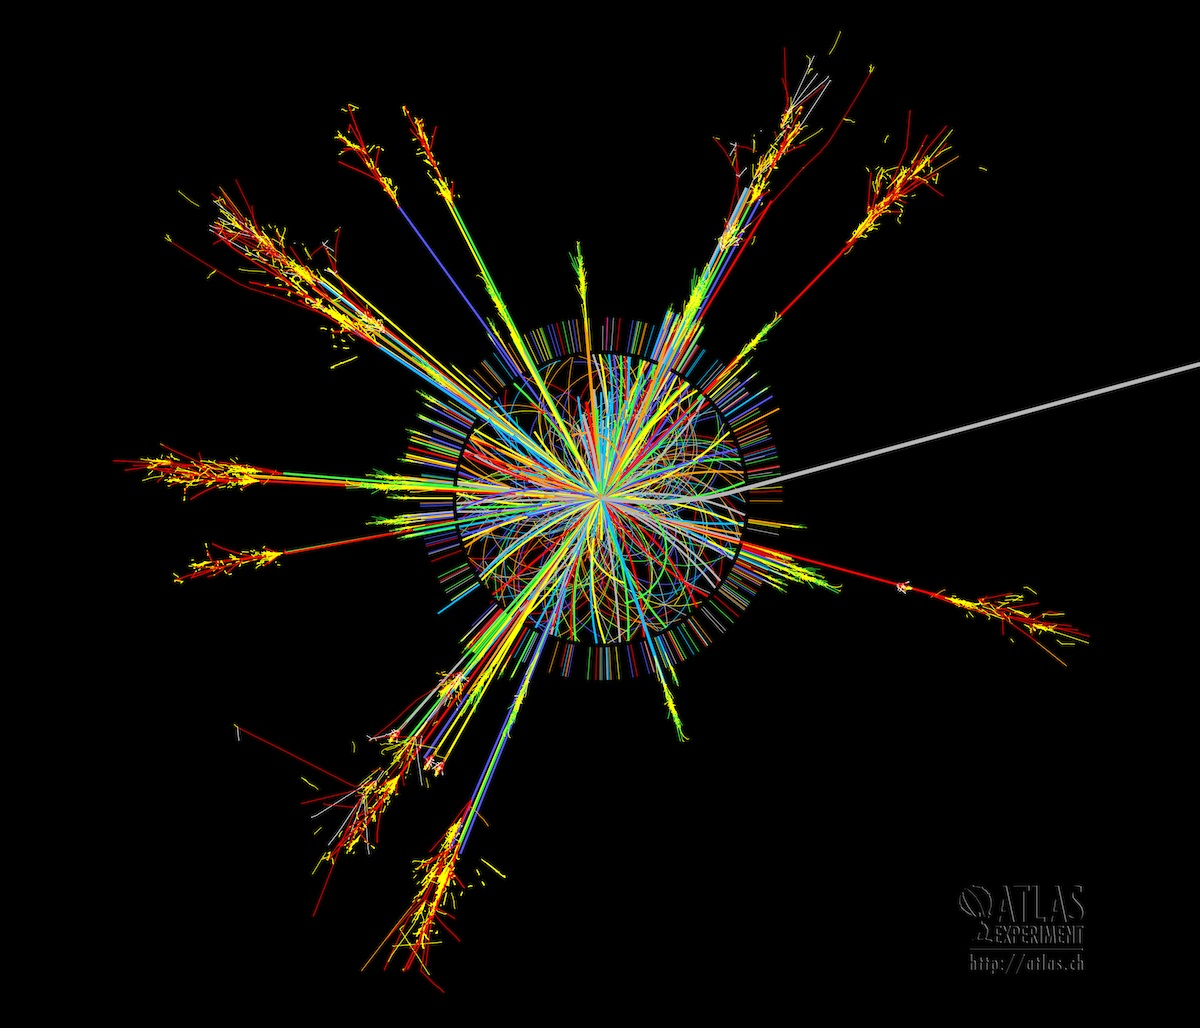
\includegraphics[width=0.3\linewidth]{HEP_event}
		\end{figure}	
	\end{minipage}
\end{columns}
\transfade[duration=.4]
\end{frame}

%------------------------------------------------
%------------------------------------------------
\section{Features in ML}
%------------------------------------------------
%------------------------------------------------

\begin{frame}[plain]
\centering
\huge

%\begin{textblock*}{0.3\paperwidth}(0.25\paperwidth,0.3\paperheight)
\centering
\vspace{0.1\paperheight}
\begin{tcolorbox}[colframe=white, colback=mygrey, width=0.4\paperwidth,
	arc=2.mm, boxsep=2mm,
	box align=center,
	halign=center,
	valign=center,
	]
	\insertsection
\end{tcolorbox}

%\end{textblock*}

\transfade[duration=.4]
\end{frame}

%------------------------------------------------

\subsection{not HEP}

\begin{frame}
\myframetitle{0.3\paperwidth}{0.04\paperwidth}{\insertsection}
\myframesubtitle{0.32\paperwidth}{\insertsubsection}

\centering
\vspace{0.2\paperheight}
\textbf{Supervised learning}
\vspace{0.05\paperheight}
\begin{columns}
	\column{0.5\textwidth}
	\centering
	\textbf{Classification}
	\begin{itemize}
		\setbeamertemplate{items}{\mybullet}
		\item cat, dog or muffin
		\item relevant or spam
		\item disease or not
        \item good or bad
        \item ...
	\end{itemize}
	
	\column{0.5\textwidth}
	\centering
	\textbf{Regression}
	\begin{itemize}
		\setbeamertemplate{items}{\mybullet}
		\item rent price
		\item temperature
		\item annual profit
        \item driving time
        \item ...
	\end{itemize}
\end{columns}

\vspace{0.1\paperheight}
Don't forget about \textbf{unsupervised learning}, \textbf{reinforcement learning}, \textbf{semi-supervised learning} and so on.

\end{frame}

%------------------------------------------------

\subsection{HEP}

\begin{frame}
\myframetitle{0.3\paperwidth}{0.04\paperwidth}{\insertsection}
\myframesubtitle{0.32\paperwidth}{\insertsubsection}

\centering
\vspace{0.2\paperheight}
\textbf{Supervised learning}
\vspace{0.05\paperheight}
\begin{columns}
	\column{0.5\textwidth}
	\centering
	\textbf{Classification}
	\begin{itemize}
		\setbeamertemplate{items}{\mybullet}
		\item b , c, uds jet
		\item $\pi$, K, $\mu$ particle
		\item t$\bar{\mathrm{t}}$ or QCD event
        \item select or reject trigger candidate
        \item ...
	\end{itemize}
	
	\column{0.5\textwidth}
	\centering
	\textbf{Regression}
	\begin{itemize}
		\setbeamertemplate{items}{\mybullet}
		\item energy resolution
		\item pile-up mitigation
        \item ...
	\end{itemize}
\end{columns}

\vspace{0.1\paperheight}
Don't forget about \textbf{unsupervised learning}, \textbf{reinforcement learning}, \textbf{semi-supervised learning} and so on.

\end{frame}

%------------------------------------------------

\subsection{ML challenges: slide 1 (A. Ustyuzhanin)}

\begin{frame}
\myframetitle{0.3\paperwidth}{0.04\paperwidth}{\insertsection}
\myframesubtitle{0.32\paperwidth}{\insertsubsection}

\centering
\vspace{0.2\paperheight}
\begin{itemize}
	\setbeamertemplate{items}{\mybullet}
	\item {Precise and fast particle tracking (single tracks, shower, jets)}
	\item {Particle identification}
	\item {Fast and accurate online data processing and filtering}
	\item {Anomaly detection (data quality monitoring, infrastructure monitoring)}
	\item {Detector design optimization (bayesian optimization, surrogate modelling)}
	\item {Data analysis (signal from background separation, ...)}
	\item {Simulation (speed-up simulation using generative models, simulator parameters optimization - tuning)}
	\item {...}
\end{itemize}

\end{frame}

%------------------------------------------------

\subsection{ML challenges: slide 2 (A. Ustyuzhanin)}

\begin{frame}
\myframetitle{0.3\paperwidth}{0.04\paperwidth}{\insertsection}
\myframesubtitle{0.32\paperwidth}{\insertsubsection}

\centering
\vspace{0.2\paperheight}
\begin{columns}
	\column{0.5\textwidth}
	\centering
	\textbf{Tracking system features}
	\begin{itemize}
		\setbeamertemplate{items}{\mybullet}
		\item Particle momentum
		\item Particle charge
		\item Track parameters
        \item Quality of track fit
        \item Number of track hits
        \item ...
	\end{itemize}
	
	\column{0.5\textwidth}
	\centering
	\textbf{RICH features}
	\begin{itemize}
		\setbeamertemplate{items}{\mybullet}
		\item Angle $\theta$
		\item Quality of angle reconstruction
		\item Reconstructed particle type
        \item Reconstructed particle energy
        \item Light intensity
        \item ...
	\end{itemize}
\end{columns}

\end{frame}

%------------------------------------------------

\subsection{ML challenges: slide 3 (A. Ustyuzhanin)}

\begin{frame}
\myframetitle{0.3\paperwidth}{0.04\paperwidth}{\insertsection}
\myframesubtitle{0.32\paperwidth}{\insertsubsection}

\centering
\vspace{0.2\paperheight}
\textbf{Calorimeter features}
\begin{itemize}
	\setbeamertemplate{items}{\mybullet}
	\item Measured particle energy
	\item Shower parameters: length, width, ...
	\item Number of clusters in each layer Intensity of the clusters
	\item Intensity of the clusters
    \item Distance form track of the original particle
    \item ...
\end{itemize}

\end{frame}

%------------------------------------------------

\subsection{ML challenges: slide 4 (A. Ustyuzhanin)}

\begin{frame}
\myframetitle{0.3\paperwidth}{0.04\paperwidth}{\insertsection}
\myframesubtitle{0.32\paperwidth}{\insertsubsection}

\centering
\vspace{0.2\paperheight}
\textbf{Muon detector features}
\begin{itemize}
	\setbeamertemplate{items}{\mybullet}
	\item Muon track parameters
	\item Quality of track fit
	\item Number of active layers
    \item Distance between the track and the active layers
    \item Length of shower
    \item ...
\end{itemize}

\end{frame}

%------------------------------------------------

\subsection{SHAP value}

\begin{frame}
\myframetitle{0.3\paperwidth}{0.04\paperwidth}{\insertsection}
\myframesubtitle{0.32\paperwidth}{\insertsubsection}

\vspace{0.2\paperheight}
\centering
	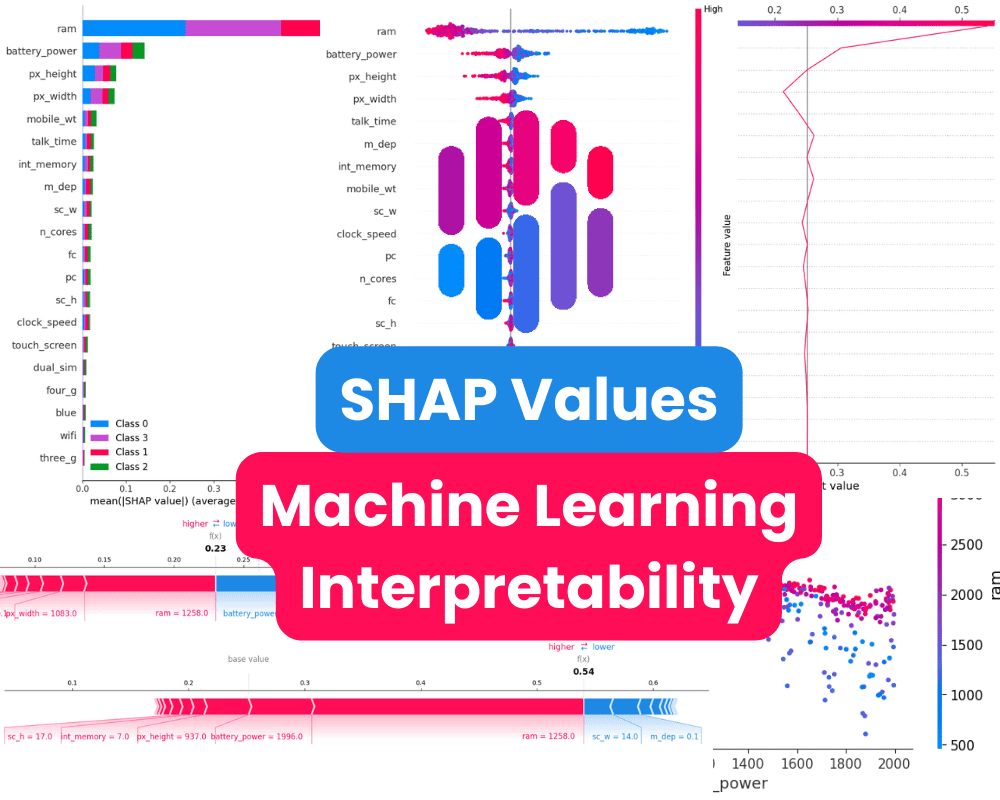
\includegraphics[width=0.6\linewidth]{shap_value.png}

\end{frame}

%------------------------------------------------
%------------------------------------------------
\section{ML pipeline}
%------------------------------------------------
%------------------------------------------------

\begin{frame}[plain]
\centering
\huge

%\begin{textblock*}{0.3\paperwidth}(0.25\paperwidth,0.3\paperheight)
\centering
\vspace{0.1\paperheight}
\begin{tcolorbox}[colframe=white, colback=mygrey, width=0.4\paperwidth,
	arc=2.mm, boxsep=2mm,
	box align=center,
	halign=center,
	valign=center,
	]
	\insertsection
\end{tcolorbox}

%\end{textblock*}

\transfade[duration=.4]
\end{frame}

%------------------------------------------------

\subsection{what is ML pipeline?}
\begin{frame}

\myframetitle{0.27\paperwidth}{0.04\paperwidth}{\insertsection}
\myframesubtitle{0.29\paperwidth}{\insertsubsection}

\vspace{0.1\paperheight}
\begin{minipage}[c][.99\textheight][t]{\linewidth}
		\centering
		\vspace{0.2\paperheight}
		\begin{figure}[t]
			\centering
			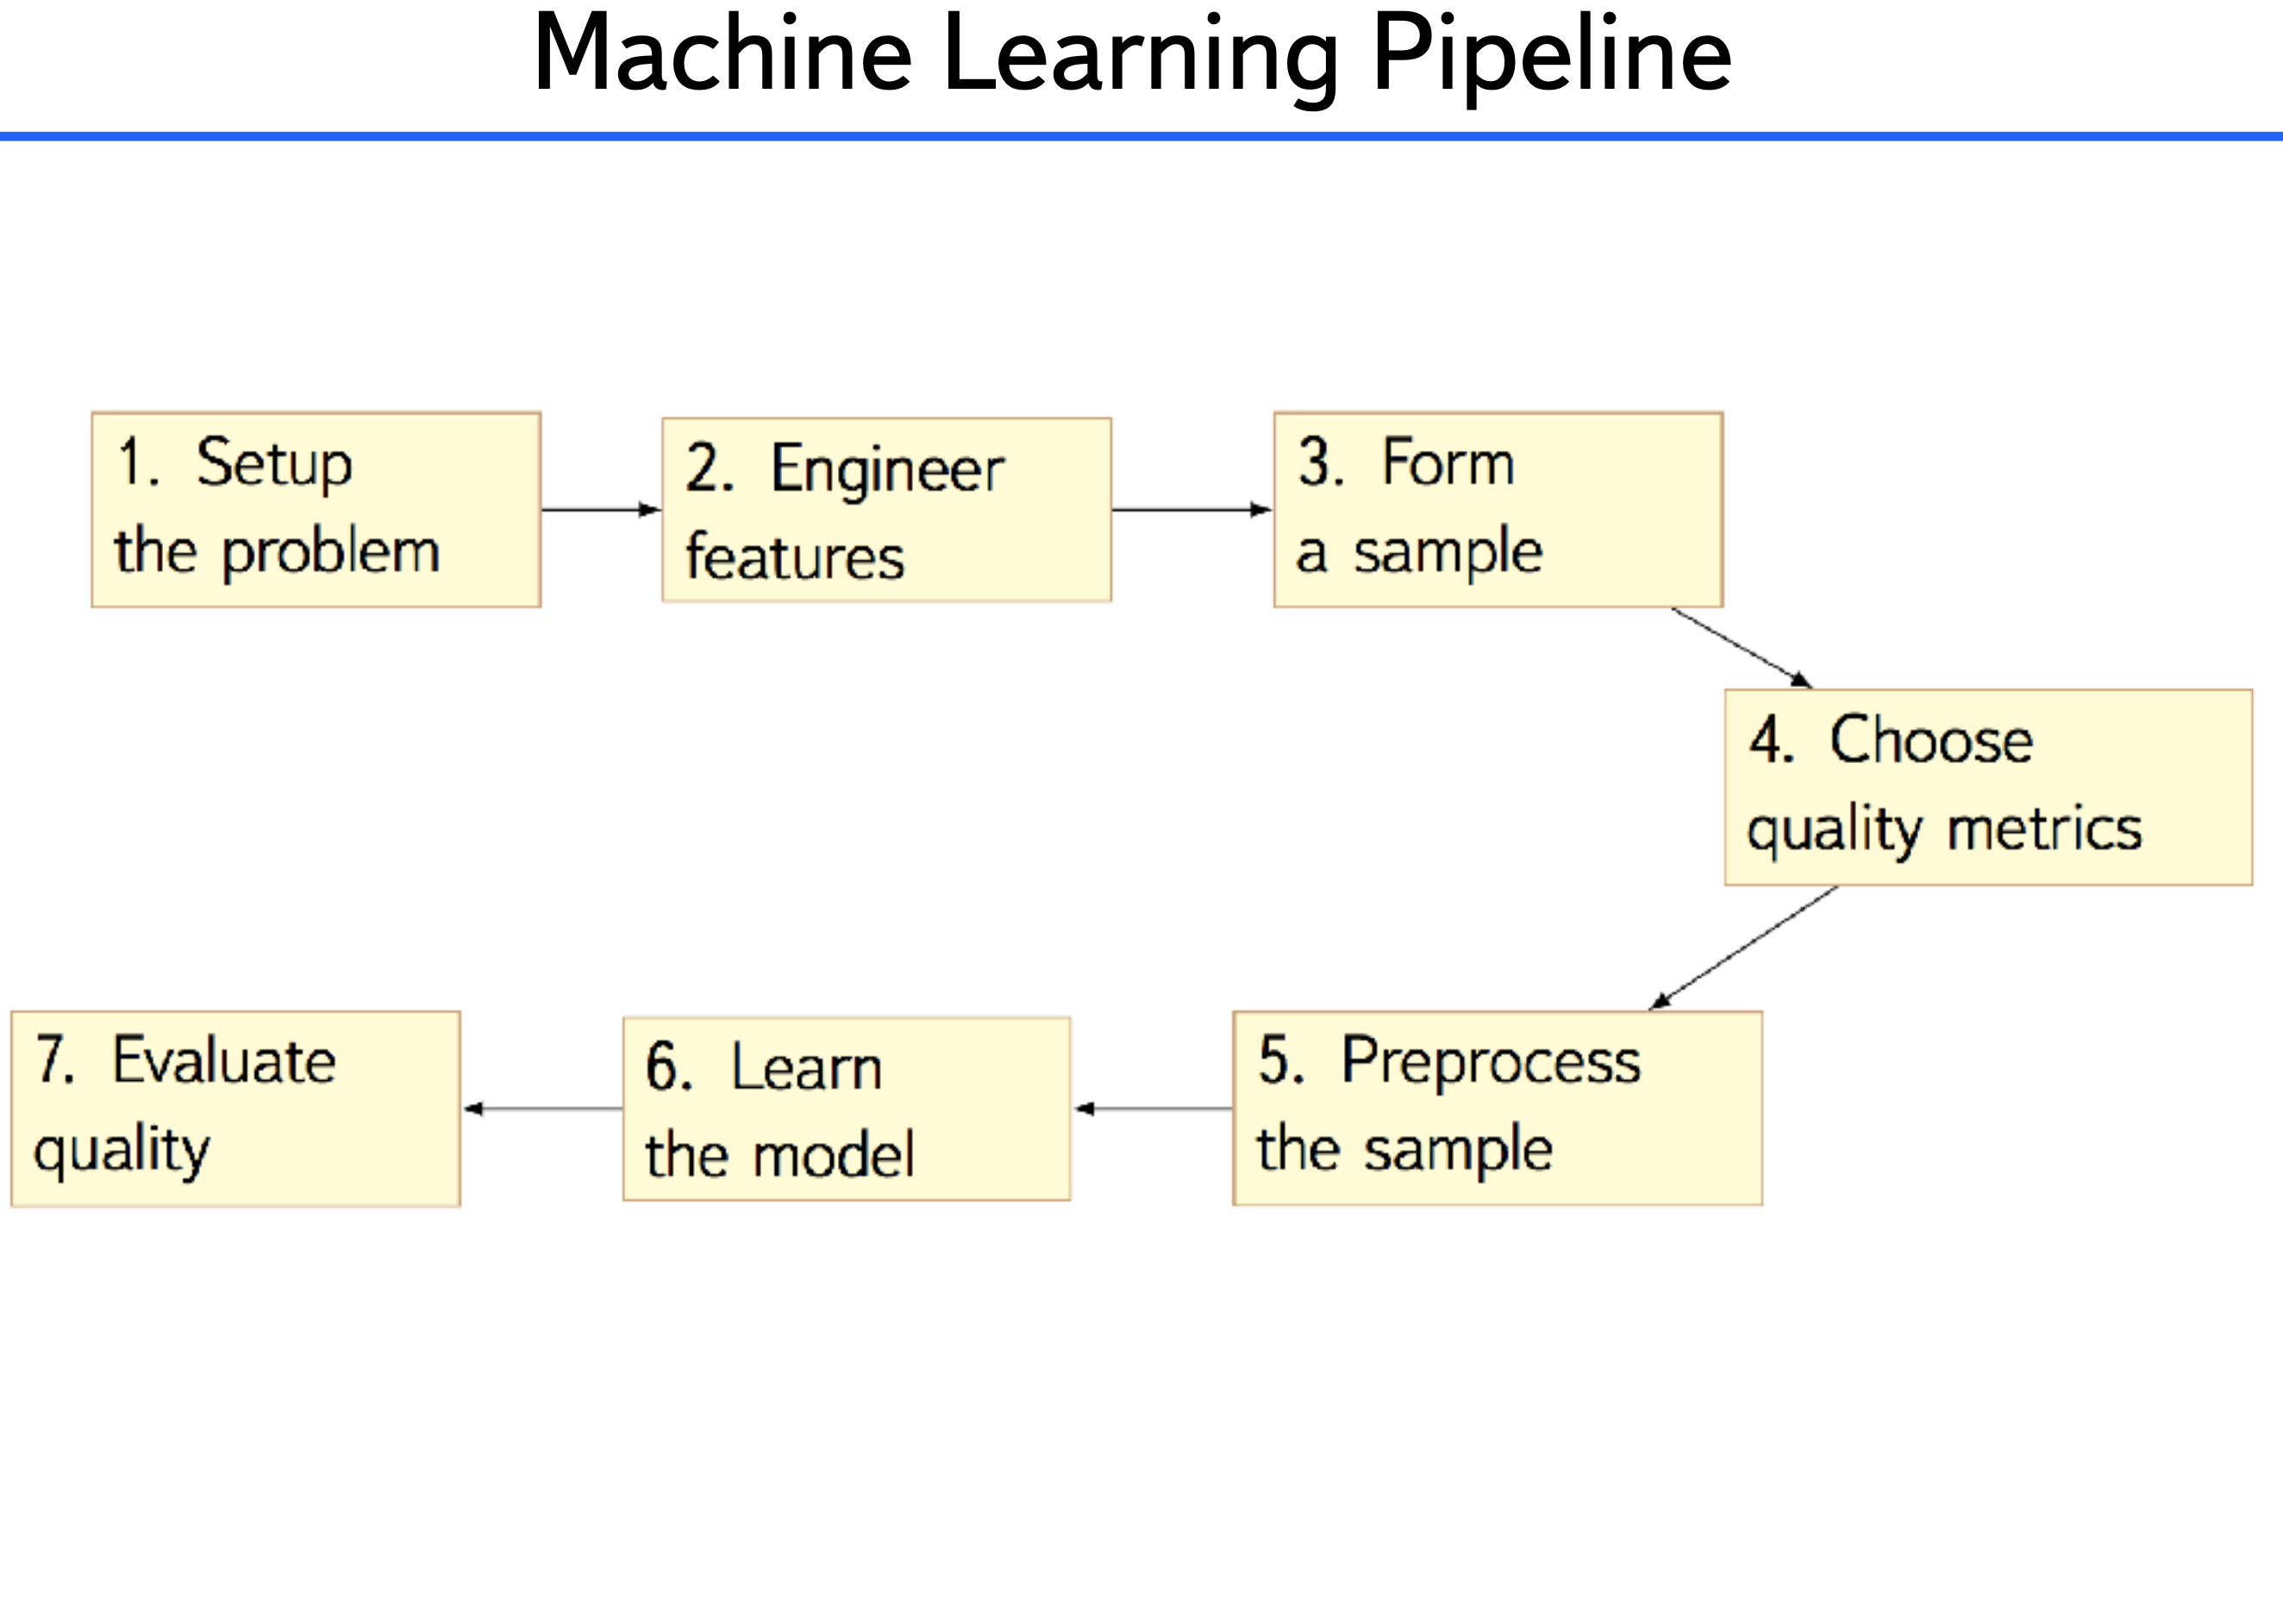
\includegraphics[width=0.448\linewidth]{pipeline1.png}
			\only<2->{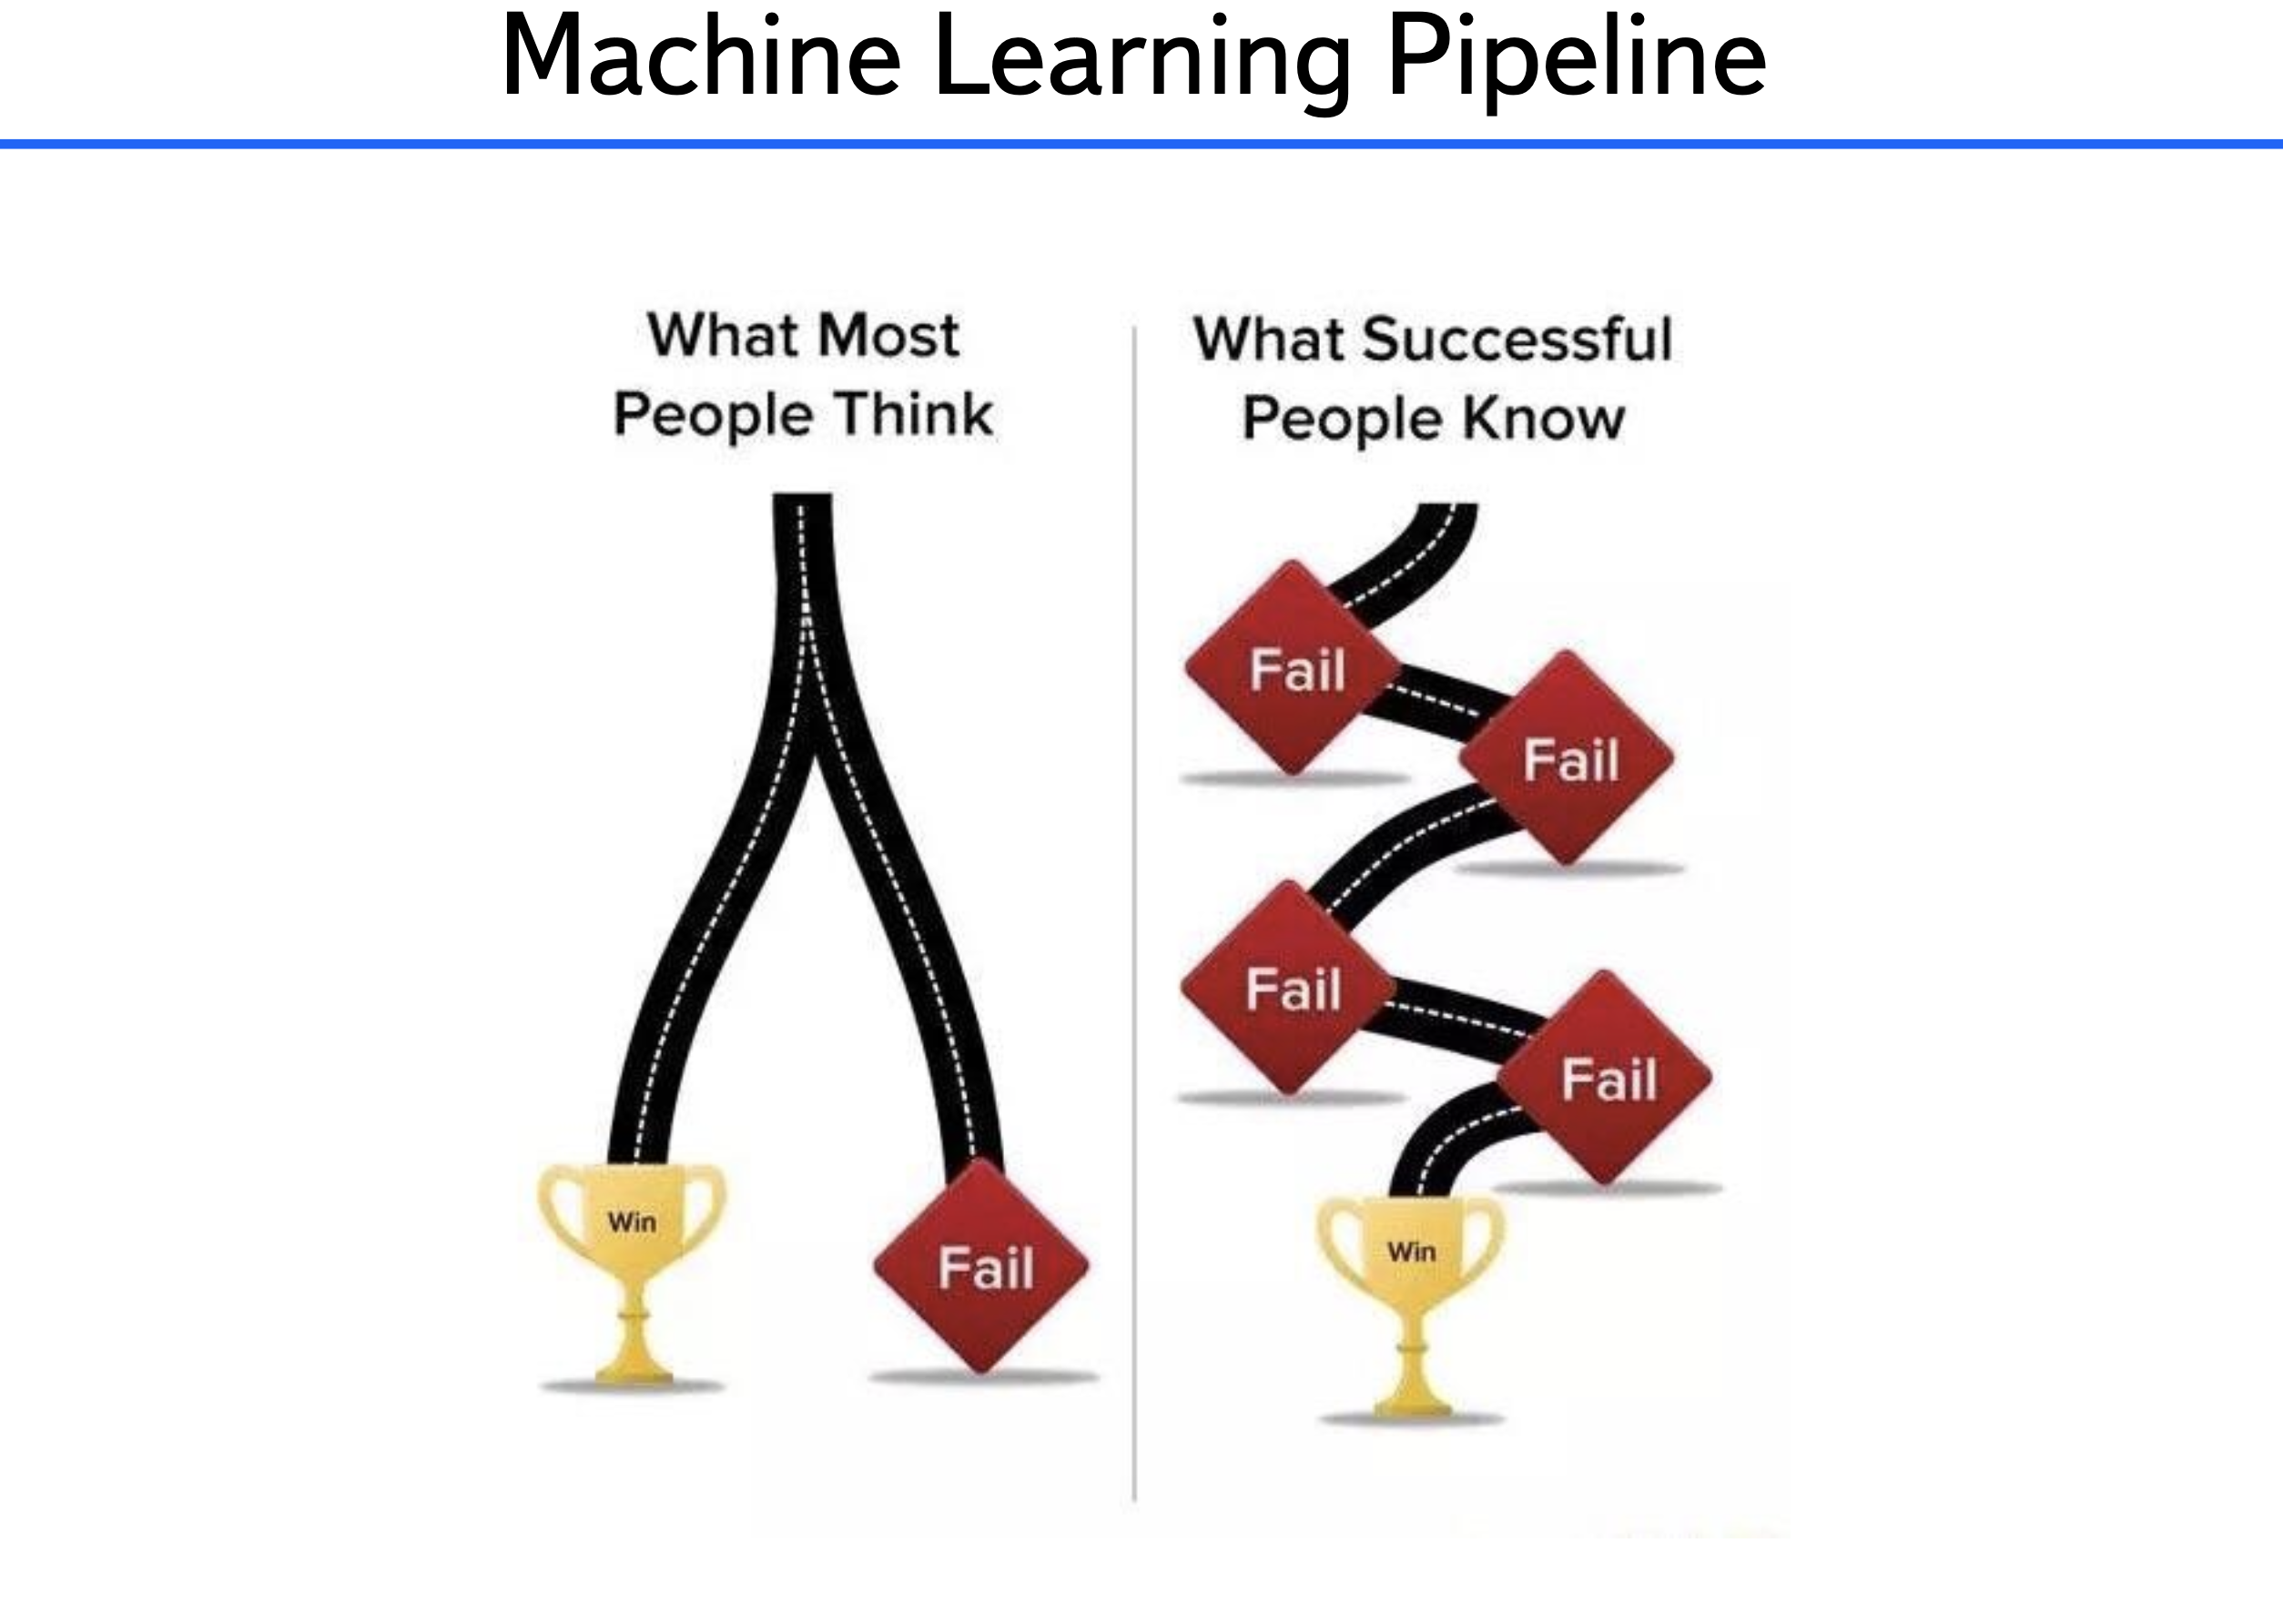
\includegraphics[width=0.45\linewidth]{pipeline2.png}}
		\end{figure}	
	\end{minipage}
\transfade[duration=.4]
\end{frame}

%------------------------------------------------
%------------------------------------------------
\section{Linear model}
%------------------------------------------------
%------------------------------------------------

\begin{frame}[plain]
\centering
\huge

%\begin{textblock*}{0.3\paperwidth}(0.25\paperwidth,0.3\paperheight)
\centering
\vspace{0.1\paperheight}
\begin{tcolorbox}[colframe=white, colback=mygrey, width=0.5\paperwidth,
	arc=2.mm, boxsep=2mm,
	box align=center,
	halign=center,
	valign=center,
	]
	\insertsection
\end{tcolorbox}

%\end{textblock*}

\transfade[duration=.4]
\end{frame}

%------------------------------------------------

\subsection{classification and regression}
\begin{frame}

\myframetitle{0.35\paperwidth}{0.04\paperwidth}{\insertsection}
\myframesubtitle{0.37\paperwidth}{\insertsubsection}

\vspace{0.2\paperheight}

\centering
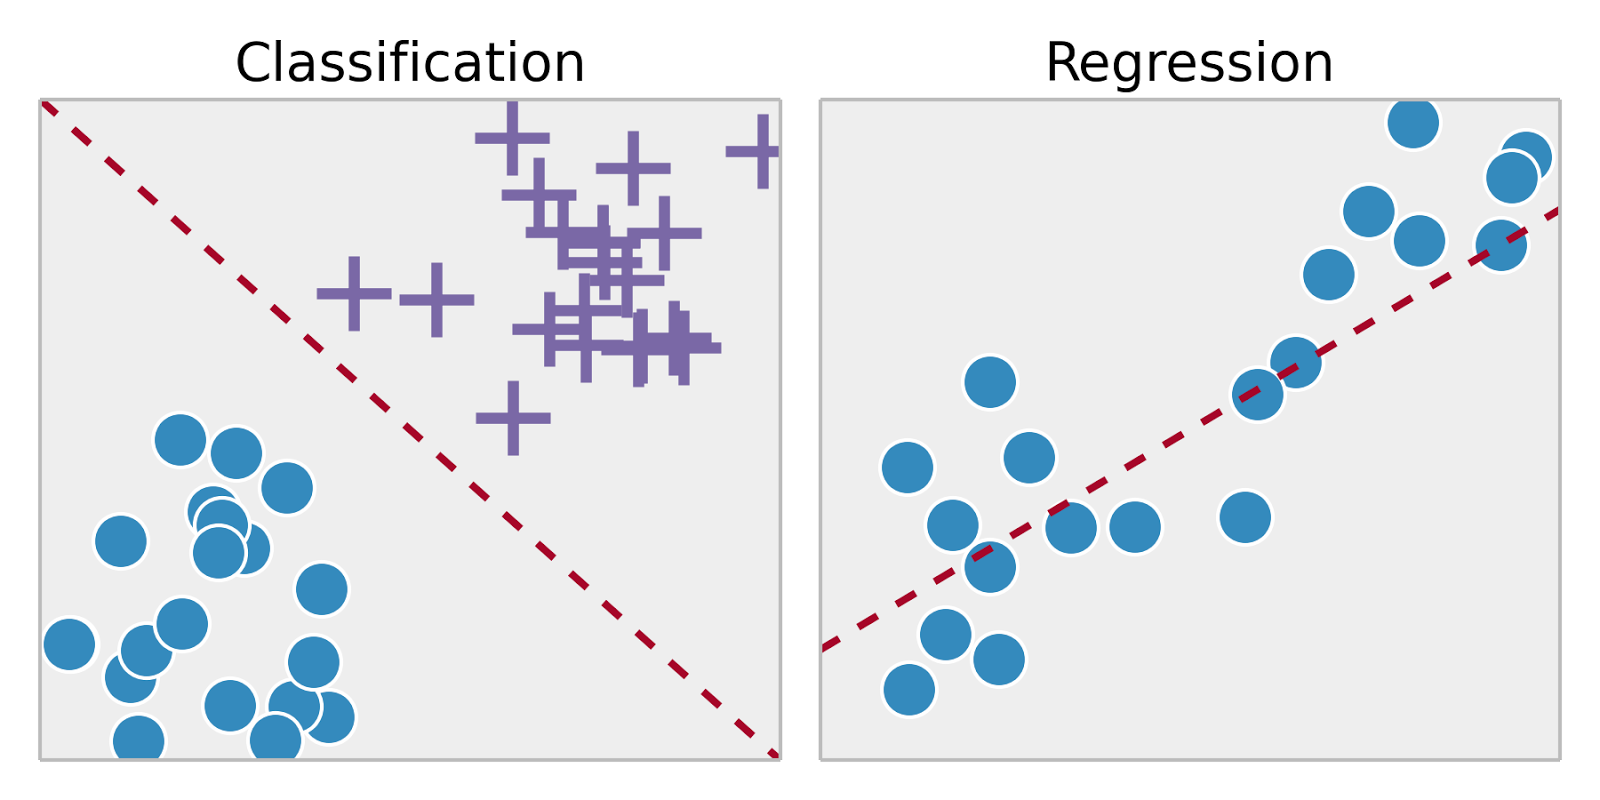
\includegraphics[width=0.8\textwidth]{linear_classification_regression.png}

\end{frame}

%------------------------------------------------

\subsection{regression}
\begin{frame}

\myframetitle{0.35\paperwidth}{0.04\paperwidth}{\insertsection}
\myframesubtitle{0.37\paperwidth}{\insertsubsection}

\vspace{0.2\paperheight}
\begin{columns}
	\column{0.55\textwidth}
	\begin{minipage}[t]{\linewidth}
		\begin{itemize}
			\item[\mybullet] $Y = \mathbb{R}$
			\item[\mybullet] N objects with K real features: $D = \mathbb{R}^K$
			\item[\mybullet] $a(\bm{x},\bm{\theta}) = \theta_0 + \sum\limits_{j=1}^{K}f_j(\bm{x})\cdot\theta_j $
			%\item[\mybullet] Extend and reassign:\\$[1, f_1(\bm{x}),\ldots ,f_K(\bm{x})] \equiv [1, x_1,\ldots ,x_K] \equiv \bm{x}$\\
			\item[\mybullet] Extend and reassign:\\$[1, f_1(\bm{x}),\ldots ,f_K(\bm{x})] \equiv \bm{x}$\\
			\vspace{0.3em}
			$[\theta_0, \ldots , \theta_K] \equiv \bm{\theta}$
			\item[\mybullet] Then $a(\bm{x},\bm{\theta}) = \langle\bm{x},\bm{\theta}\rangle$
		\end{itemize}
	\end{minipage}%	
	\column{0.5\textwidth}
	\begin{minipage}[c]{\linewidth}
		\centering
	
		\begin{itemize}
			\item[\mybullet] Minimization problem:
			\begin{itemize}
				\normalsize
				\item[\mysubbullet] $\mathcal{L}(\bm \theta) = \big(\langle\bm{x},\bm{\theta}\rangle - y\big)^2$
				\item[\mysubbullet] $Q(\bm{\theta}) = \frac{1}{N}\sum\limits_{i=1}^{N}\big(\langle\bm{x_i},\bm{\theta}\rangle - y_i\big)^2$
			\end{itemize}
			\item[\mybullet] Then we need to minimize $Q(\bm{\theta})$ by varying $\bm\theta$:
			\vspace{1mm}
			\begin{itemize}
				\normalsize
				\item[\mysubbullet] $\hat{a}=\text{arg}~ \underset{\bm{\theta} \in \Theta}{\text{min}}~Q(\bm{\theta})$
			\end{itemize}
			
		\end{itemize}	
	\end{minipage}
\end{columns}

\end{frame}

%------------------------------------------------

\subsection{classification}
\begin{frame}

\myframetitle{0.35\paperwidth}{0.04\paperwidth}{\insertsection}
\myframesubtitle{0.37\paperwidth}{\insertsubsection}

\vspace{0.2\paperheight}
\begin{columns}
	\column{0.55\textwidth}
	\begin{minipage}[t]{\linewidth}
		\begin{itemize}
			\item[\mybullet] $Y = \{-1, +1\}$
			\item[\mybullet] N objects with K real features: $D = \mathbb{R}^K$
			\item[\mybullet] $a(\bm{x},\bm{\theta}) = \theta_0 + \sum\limits_{j=1}^{K}f_j(\bm{x})\cdot\theta_j $
			\item[\mybullet] Extend and reassign:\\$[1, f_1(\bm{x}),\ldots ,f_K(\bm{x})] \equiv [1, x_1,\ldots ,x_K] \equiv \bm{x}$\\
			$[\theta_0, \ldots , \theta_K] \equiv \bm{\theta}$
			\item[\mybullet] Then $a(\bm{x},\bm{\theta}) = \langle\bm{x},\bm{\theta}\rangle$
		\end{itemize}
	\end{minipage}%	
	\column{0.5\textwidth}
	\begin{minipage}[c]{\linewidth}
		\centering
		
		\begin{itemize}
			\item[\mybullet] Minimization problem:
			\begin{itemize}
				\normalsize
				\item[\mysubbullet] $\mathcal{L}(\bm \theta) = \bigl[\text{sign}\langle\bm{x},\bm{\theta}\rangle \neq y\bigr]$
				\item[\mysubbullet] $Q(\bm{\theta}) = \frac{1}{N}\sum\limits_{i=1}^{N}\bigl[\text{sign}\langle\bm{x_i},\bm{\theta}\rangle \neq y_i\bigr]$
			\end{itemize}
			\item[\mybullet] Then we need to minimize $Q(\bm{\theta})$ by varying $\bm\theta$:
			\vspace{1mm}
			\begin{itemize}
				\normalsize
				\item[\mysubbullet] $\hat{a}=\text{arg}~ \underset{\bm{\theta} \in \Theta}{\text{min}}~Q(\bm{\theta})$
			\end{itemize}
			
		\end{itemize}	
	\end{minipage}
\end{columns}

\end{frame}

\end{document}
